\documentclass[border=1pt,tikz,varwidth=\maxdimen]{standalone}

\usetikzlibrary{positioning,calc,arrows.meta,trees}

\usepackage{amsmath,mathtools}

\begin{document}

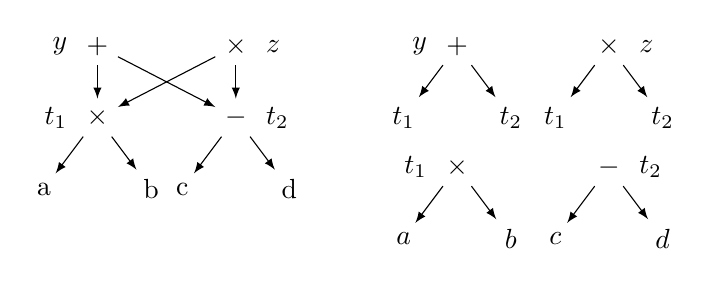
\begin{tikzpicture}[
  level distance=6ex,
  sibling distance=9ex,
  array/.style={edge from parent/.style={solid,draw,-latex}},
  empty/.style={edge from parent/.style={}},
  narrow/.style={sibling distance=5ex},
  ]
  \coordinate (y);
  \node [below=1ex of y] (y-add) {\(+\)}
  child [array] {
    node (t1-times) {\(\times\)}
    child {
      node {a}
    }
    child {
      node {b}
    }
  };
  \coordinate [right=5em of y] (z);
  \node [below=1ex of z] (z-times) {\(\times\)}
  child [array] {
    node (t2-sub) {\(-\)}
    child {
      node {c}
    }
    child {
      node {d}
    }
  };
  \node [left=0ex of y-add] {\(y\)};
  \node [left=0ex of t1-times] {\(t_{1}\)};
  \node [right=0ex of z-times] {\(z\)};
  \node [right=0ex of t2-sub] {\(t_{2}\)};
  \draw [-latex] (y-add) -- (t2-sub);
  \draw [-latex] (z-times) -- (t1-times);

  \coordinate [right=8em of z] (tree);
  \node [below=1ex of tree] (y-tree) {\(+\)}
  child [array] {
    node {\(t_{1}\)}
  }
  child [array] {
    node {\(t_{2}\)}
  };
  \node [below=3em of y-tree] (t1-tree) {\(\times\)}
  child [array] {
    node {\(a\)}
  }
  child [array] {
    node {\(b\)}
  };
  \node [right=4em of y-tree] (z-tree) {\(\times\)}
  child [array] {
    node {\(t_{1}\)}
  }
  child [array] {
    node {\(t_{2}\)}
  };
  \node [below=3em of z-tree] (t2-tree) {\(-\)}
  child [array] {
    node {\(c\)}
  }
  child [array] {
    node {\(d\)}
  };
  \node [left=0ex of y-tree] {\(y\)};
  \node [left=0ex of t1-tree] {\(t_{1}\)};
  \node [right=0ex of z-tree] {\(z\)};
  \node [right=0ex of t2-tree] {\(t_{2}\)};
\end{tikzpicture}

\end{document}
